%!TEX root = thesis.tex

\chapter{State of the art}
\label{chapter:stateofart}


This dissertation is concerned with the scalability and optimization of EAC to large datasets.
The goal of this optimization is to elevate the EAC method to large datasets, which translates in optimizing both speed and space.
To this end, several aspects were researched.
Work related to clustering and the concept of big data was briefly reviewed in section \ref{sec:big data}.


Evidence Accumulation Clustering is a method of three parts.
This dissertation is concerned with the scalability of the whole algorithm which means that different steps have to be optimized separately.
This algorithm and existing work on its scalability is reviewed in section \ref{sec:eac}.
The first step is the generation of an ensemble of clustering partitions.
Increasing speed can be attained with either faster algorithms and/or faster computation of existing algorithms.
Both these approaches to faster generation of the ensemble were pursued and researched.
The former in the form of the still young field of quantum clustering, which is briefly reviewed in section \ref{sec:quantum clustering}, and the later in the field of parallel computation, more specifically on computation in GPUs, reviewed in section \ref{sec:gpgpu}.
While quantum clustering was only reviewed for the first step, the parallel computation paradigm was investigated with all steps in mind.
For that reason, K-Means GPU versions were researched as well as Hierarchical Agglomerative Clustering.


%TODO double check all refs because this was merged pre latex citations and the reference might have gotten mixed

%TODO
% see if this is an apropriate structure; a quantum clustering section makes sense at the very least, but it should be introduced before

\section{Quantum clustering}
\label{sec:quantum clustering}
The field of quantum clustering has shown promising results regarding potential speedups in several tasks over their classical counterparts. 
There are two major paths for the problem of quantum clustering. The first is the quantization of clustering methods to work in quantum computers. This translates in converting algorithms to work partially or totally on a different computing paradigm, with support of quantum circuits or quantum computers. Literature suggests that quadratic (and even exponential in some cases) speedup may be achieved. Most of the approaches for such conversions make use of Groover's search algorithm, or a variant of it, e.g. \citet{Wiebe2014}. Most literature on this path is also mostly theoretical since quantum circuits are not easily available and a working quantum computer has yet to be invented. This path can be seen as part of the bigger problem of quantum computing and quantum information processing.

% #TODO get refs for simulation of quantum systems not being feasable; Feynmann; I think washington course had something -->

An alternative to using real quantum systems would be to simulate them. However, simulating quantum systems in classical computers is a very hard task by itself and literature suggest is not feasible. Given that the scope of the thesis is to accelerate clustering, having the extra overhead of simulating the systems would not allow speedups.

The second approach is the computational intelligence approach, i.e.  to use algorithms that muster inspiration from quantum analogies. A study of the literature will reveal that this path typically further divides itself into two approaches. One comprehends the algorithms based on the concept of the qubit, the quantum analogue of a classical bit with interesting properties found in quantum objects. The other approach models data as a quantum system and uses the Schrödinger equation to evolve it.

In the following two sections these approaches for quantum inspired computational intelligence are explored.

\subsection{The quantum bit approach}
\label{sec:qubit}

\subsubsection{What is a quantum bit?}

To understand the workings of the algorithms based on the concept of the qubit, it is useful to cast some insight about its properties and functioning.
The quantum bit is a quantum object that has the properties of quantum superposition, entanglement and ...

% taken from notebook -->

A qubit can have any value between 0 and 1 (superposition property) until it is observed, which is when the system collapses to either state. However, the probability with which the system collapses to either state  may be different. The superposition property or linear combination of states can be expressed as

$$
[\psi] = \alpha[0] + \beta[1]
$$

where $\psi$ is an arbitrary state vector and $\alpha$, $\beta$ are the the probability amplitude coefficients of basis states $[0]$ and $[1]$, respectively. The basis states correspond to the spin of the modelled particle (in this case, a ferminion, e.g. electron). The coefficients are subjected to the following normalization:

$$|\alpha|^2 + |\beta|^2 = 1$$

where $|\alpha|^2$, $|\beta|^2$ are the probabilities of observing states $[0]$ and $[1]$, respectevely. $\alpha$ and $\beta$ are complex quantities and represent a qubit:

$$\begin{bmatrix}
\alpha \\
\beta
\end{bmatrix}$$

Moreover, a qubit string may be represented by:
$$
\begin{bmatrix}
\left.\begin{matrix}
\alpha_1\\ 
\beta_1
\end{matrix}\right| & \left.\begin{matrix}
\alpha_2\\ 
\beta_2
\end{matrix}\right| & \begin{matrix}
\alpha_3\\ 
\beta_3
\end{matrix}
\end{bmatrix}
$$

The probability of observing the state $[000]$ will be $|\alpha_1|^2 \times |\alpha_2|^2 \times |\alpha_3|^2$
To use this model for computing purposes, black-box objects called \emph{oracles} are used.

% end of notebook -->

% #TODO get ref -->
Def from wiki: In complexity theory and computability theory, an oracle machine is an abstract machine used to study decision problems. It can be visualized as a Turing machine with a black box, called an oracle, which is able to decide certain decision problems in a single operation. The problem can be of any complexity class. Even undecidable problems, like the halting problem, can be used. %from http://en.wikipedia.org/wiki/Oracle_machine




\subsubsection{Quantum K-Means}

Several clustering algorithms ~\cite{Casper2013,Casper,Xiao2010}, as well as optimization problems ~\cite{Wang2013}, are modelled after this concept. To test the potential of the algorithms under this paradigm, a quantum variant of the K-Means algorithm based on~\cite{Casper} was chosen as a case study.

\subsubsection{Description of the algorithm}

The Quantum K-Means (QK-Means) algorithm, as is described in ~\cite{Casper}, is based on the classical K-Means algorithm. It extends the basic K-Means with concepts from quantum mechanics (the qubit) and genetic algorithms.

Within the context of this algorithm, oracles contain strings of qubits and generate their own input by observing the state of the qubits. After collapsing, the qubit value becomes analogue to a classical bit.

%#TODO get ref : see washington quantum computing classes -->

Ideally, oracles would contain actual quantum systems or simulate them - this would correctly account for the desirable quantum properties. As it stands, oracles aren't quantum systems or even simulate them. The most appropriate description would be a probabilistic Turing machine.
Each string of qubits represents a number, so the number of qubits in each string will define its precision. The number of strings chosen for the oracles depends on the number of clusters and dimensionality of the problem (e.g. for 3 clusters of 2 dimensions, 6 strings will be used since 6 numbers are required). Each oracle will represent a possible solution.

% (describe algorithm... - from notebook) -->
The algorithm has the following steps:
\begin{enumerate}
\item Initialize population of oracles
\item Collapse oracles
\item K-Means
\item Compute cluster fitness
\item Store
\item Quantum Rotation Gate
\item Collapse oracles
\item Quantum cross-over and mutation
\item Repeat 3-7 until generation (iteration) limit is reached
\end{enumerate}


\paragraph{Initialize population of oracles}

The oracles are created in this step and all qubit coefficients are initialized with $\frac{1}{\sqrt{2}}$, so that the system will observe either state with equal probability. This value is chosen taken into account the necessary normalization of the coefficients.

\paragraph{Collapse oracles}

Collapsing the oracles implies making an observation of each qubit of each qubit string in each oracle. This is done by first choosing a coefficient to use (either can be used), e.g. $\alpha$. Then, a random value $r$ between 0 and 1 is generated. If $\alpha \ge r$ then the system collapses to $[0]$, otherwise to $[1]$.

\paragraph{K-Means}
In this step we convert the binary representation of the qubit strings to base 10 and use those values as initial centroids for K-Means. For each oracle, classical K-Means is then executed until it stabilizes or reaches the iteration limit. The solution centroids are returned to the oracles in binary representation.

\paragraph{Compute cluster fitness}
Cluster fitness is computed using the Davies-Bouldin index for each oracle. The score of each oracle is stored in the oracle itself.

\paragraph{Store}
The best scoring oracle is stored.

\paragraph{Quantum Rotation Gate}
So far, the algorithm consisted of the classical K-Means with a complex random number generation for the centroids and complicated data structures. This is the step that fundamentally differs from the classical version. In this step a quantum gate (in this case a rotation gate) is applied to all oracles except the best one. The basic idea is to shift the qubit coefficients of the least scoring oracles so they'll have a higher probability of collapsing into initial centroid values closer to the best solution so far. This way, in future generations, we'll not initiate with the best centroids so far (which will not converge further into a better solution) but we'll be closer while still ensuring diversity (which is also a desired property of the genetic computing paradigm). In other words, we look for better solutions than the one we got before in each oracle while moving in the direction of the best we found so far.

% (end of notebook entry) -->

The genetic operations of cross-over and mutation are both part of the genetic algorithms toolbox. \cite{Wiebe2014} suggests that that this operations may not be required to produce variability in the population of qubit strings. This is because, according to \cite{Liu2010}, use of the angle-distance rotation method in the quantum rotation operation produces enough variability, with a careful choice of the rotation angle. However, if they were used, their goal is to produce further variability into the population of qubit strings.


%TODO
% add ref

\subsection{Horn and Gottlieb's algorithm}
\label{sec:horn}

The other approach to clustering that gathers inspiration from quantum mechanical concepts is to use the Schrödinger equation. The algorithm under study was created by Horn and Gottlieb and was later extended by Weinstein and Horn.

The first step in this methodology is to compute a probability density function of the input data. This is done with a Parzen-window estimator in ~\cite{Horn2001a,Weinstein2009}.
The Parzen-window density estimation of the input data is done by associating a Gaussian with each point, such that

$$ \psi (\mathbf{x}) = \sum ^N _{i=1} e^{- \frac{\left \| \mathbf{x}-\mathbf{x}_i \right \| ^2}{2 \sigma ^2}} $$

where $N$ is the total number of points in the dataset, $\sigma$ is the variance and $\psi$ is the probability density estimation. $\psi$ is chosen to be the wave function in Schrödinger's equation. The details of why this is are better described in ~\cite{Weinstein2009,Horn2001a,Horn2001b}.

Having this information we'll compute the potential function $V(x)$ that corresponds to the state of minimum energy (ground state = eigenstate with minimum eigenvalue) ~\cite{Horn2001a}, by solving the Schrödinger's equation in order of $V(x)$:      

$$
V(\mathbf{x}) = E + \frac {\frac{\sigma^2}{2}\nabla^2 \psi }{\psi} 
= E - \frac{d}{2} + \frac {1}{2 \sigma^2 \psi} \sum ^N _{i=1} \left \| \mathbf{x}-\mathbf{x}_i \right \| ^2 e^{- \frac{\left \| \mathbf{x}-\mathbf{x}_i \right \| ^2}{2 \sigma ^2}}
$$

And since the energy should be chosen such that $\psi$ is the groundstate (i.e. eigenstate corresponding to minimum eigenvalue) of the Hamiltonian operator associated with Schrödinger's equation (not represented above), the following is true

$$
E = - min \frac {\frac{\sigma^2}{2}\nabla^2 \psi }{\psi}
$$

With all of this, $V(x)$ can be computed.
This potential function is akin to the inverse of a probability density function. Minima of the potential correspond to intervals in space where points are together. So minima will naturally correspond to cluster centres ~\cite{Horn2001a}.
However, it's very computationally intensive to compute $V(x)$ to the whole space, so we only compute the value of this function at the data points.
This should not be problematic since clusters' centres are generally close to the data points themselves. 
Even so, the minima may not lie on the data points themselves.
One method to address this problem is to compute the potential on the input data and converge this points toward some minima of the potential function. This is done with the gradient descent method in ~\cite{Horn2001a}. 

Another method ~\cite{Weinstein2009} is to think of the input data as particles and use the Hamiltonian operator to evolve the quantum system in the time-dependant Schrödinger equation. Given enough time steps, the particles will converge to and oscillate around potential minima. This method makes the Dynamic Quantum Clustering algorithm.
The nature of the computations involved in this algorithm make it a good candidate for parallelization techniques. \cite{Wittek2013} parallelized this algorithm to the GPU obtaining speedups of up to two magnitudes relative to an optimized multicore CPU implementation.

% #TODO describe the fine cluster algorithm; critique how this is done; what was developed; what  -->


%[1] N. Wiebe, A. Kapoor, and K. Svore, “Quantum Algorithms for Nearest-Neighbor Methods for Supervised and Unsupervised Learning,” p. 31, 2014.
%
%~\cite{Wiebe2014}

%[2] D. Horn and A. Gottlieb, “The Method of Quantum Clustering.,” NIPS, no. 1, 2001.
%~\cite{Horn2001a}

%[3] M. Weinstein and D. Horn, “Dynamic quantum clustering: a method for visual exploration of structures in data,” Phys. Rev. E - Stat. Nonlinear, Soft Matter Phys., vol. 80, no. 6, pp. 1–15, Dec. 2009.
%~\cite{Weinstein2009}

%[4] E. Casper and C. Hung, “Quantum Modeled Clustering Algorithms for Image Segmentation,” vol. 2, no. March, pp. 1–21, 2013.
%~\cite{Casper2013}
%
%[5] E. Casper, C.-C. Hung, E. Jung, and M. Yang, “A Quantum-Modeled K-Means Clustering Algorithm for Multi-band Image Segmentation.” [Online]. Available: http://delivery.acm.org/10.1145/2410000/2401639/p158-casper.pdf?ip=193.136.132.10&id=2401639&acc=ACTIVE SERVICE&key=2E5699D25B4FE09E.F7A57B2C5B227641.4D4702B0C3E38B35.4D4702B0C3E38B35&CFID=476955365&CFTOKEN=55494231&__acm__=1423057410_0d77d9b5028cb3. [Accessed: 04-Feb-2015].

%~\cite{Casper}

%[6] J. Xiao, Y. Yan, J. Zhang, and Y. Tang, “A quantum-inspired genetic algorithm for k-means clustering,” Expert Syst. Appl., vol. 37, pp. 4966–4973, 2010.
%~\cite{Xiao2010}

%
%[7] H. Wang, J. Liu, J. Zhi, and C. Fu, “The Improvement of Quantum Genetic Algorithm and Its Application on Function Optimization,” vol. 2013, no. 1, 2013.
%~\cite{Wang2013}

%
%[8] W. Liu, H. Chen, Q. Yan, Z. Liu, J. Xu, and Y. Zheng, “A novel quantum-inspired evolutionary algorithm based on variable angle-distance rotation,” 2010 IEEE World Congr. Comput. Intell. WCCI 2010 - 2010 IEEE Congr. Evol. Comput. CEC 2010, 2010.
%~\cite{Liu2010}



\section{Evidence Accumulation Clustering}
\label{sec:eac}

\subsection{Ensemble Clustering}


\paragraph{Ensemble clustering}
Data from real world problems appear in different configurations regarding shape, size, sparsity, etc. %taken from Fred(2005)
Different clustering algorithms are appropriate for different data configurations, e.g. K-Means using euclidean distance as metric tends to group patterns in hyperspheres so it is more appropriate for data whose structure is formed by hypershere like clusters.%TODO see http://cstheory.stackexchange.com/questions/17693/hyperspherical-nature-of-k-means-and-similar-clustering-methods for paper reference and justification
If the true structure of the data at hand is heterogeneous in configuration, a single clustering algorithm might perform well for some part of the data while other performs better for some other part. The underlying idea behind ensemble clustering is to use multiple clusterings from one or more clustering algorithms and combine them in such a way that the final clustering is better than any of the individual ones.

\paragraph{Formulation}
Some notation and nomenclature, adopted from ~\cite{Fred2005}, should be defined since it will be used throughout the remainder of the present work. The term \emph{data} refers to a set $X$ of $n$ objects or patterns $X=\left \{ \textsc{x}_1,...,\textsc{x}_n \right \}$, and may be represented by $\chi = \left \{ x_1,...,x_n \right \}$, such that $x_i \in  \mathbb{R}^d$. A clustering algorithm takes $\chi$ as input and returns $k$ groups or \emph{clusters} $C$ of some part of the data, which form a \emph{partition} $P$. A clustering \emph{ensemble} $\mathbb{P}$ is group of such partitions. This means that:

$$
\mathbb{P} = \left \{   P^1, P^2, ... P^N   \right \} \\
P^j = \left \{   \textsc{x}^j_1, \textsc{x}^j_2, ... \textsc{x}^{j}_{k_j}   \right \} \\
C^j_k = \left \{   x_a, x_b, ..., x_z   \right \}
$$

\subsection{Overview of Evidence Accumulation Clustering} 
The Evidence Accumulation Clustering makes no assumption on the number of clusters in each data partition. Its approach is divided in 3 steps:

\begin{enumerate}
\item Produce a clustering ensemble $\mathbb{P}$ (the evidence)
\item Combine the evidence
\item Recover natural clusters 
\end{enumerate}

A clustering ensemble, according to ~\cite{Fred2005}., can be produced from (1) different data representations, e.g. choice of preprocessing, feature extraction, sampling; or (2) different partitions of the data, e.g. output of different algorithms, varying the initialization parameters on the same algorithm.

The ensemble of partitions is combined in the second step, where a non-linear transformation turns the ensemble into a co-association matrix, i.e. a matrix $C$ where each of its elements $n_{ij}$ is the association value between the object pair $(i,j)$. The association between any pair of patterns is given by the number of times those two patterns appear clustered together in any cluster of any partition of the ensemble. The rationale is that pairs that are frequently clustered together are more likely to be representative of a true link between the patterns ~\cite{Fred2005}, revealing the underlying structure of the data.
The construction of this matrix is at the very core of this method.

The co-association matrix itself doesn't output a clustering partition. Instead, it is used as input to other methods to obtain the final partition. Since this matrix is a similarity matrix it's appropriate to use in algorithms take this type of matrices as input, e.g. K-Medoids or hierarchical algorithms such as Single-Link. to name two. Typically, algorithms use a distance as the similarity, which means that they minimize the values of similarity to obtain the highest similarity between objects. However, a low value on the co-association matrix translates in a low similarity between a pair of objects, which means that the co-association matrix requires prior transformation for accurate clustering results, e.g. replace every similarity value $n_{ij}$ between every pair of object $(i,j)$ by $max \{ C \} - n_{ij}$.


\paragraph{Examples of applications}

EAC has been used with success in several applications:
\begin{itemize}
	\item in the field of bioinformatics it was used for the automatic identification of chronic lymphocyt leukemia \cite{Qian2010};
	\item also in bioinformatics it was used for the unsupervised analysis of ECG-based biometric database to highlight natural groups and gain further insight \cite{Lourenco2009};
	\item in computer vision it was used as a solution to the problem of clustering of contour images (from hardware tools) \cite{Lourenco2007}.
\end{itemize}



\paragraph{advantages}

\paragraph{disadvantages}
quadratic space and time complexities because of the nxn co-association matrix 


\subsection{Scalability of EAC} 
The quadratic space and time complexity of processing the $n \times n$ co-association matrix is an obstacle to an efficient scaling of EAC. Two approaches have been proposed to address this obstacle: one dealing reducing the co-association matrix by considering only the distances of patterns to theirs $p$ neighbours and the other by maximizing the sparsity of the co-association matrix.

\subsubsection{$p$ neighbours approach}
The first approach, \cite{Fred2005}, proposes an alternative $n \times p$ co-association matrix, where only the $p$ nearest neighbours of each sample are considered in the voting mechanism. This comes at the cost of having to keep track of the neighbours of each pattern in a separate data structure and also of pre-computing the $p$ neighbours. Still, considering that the quadratic space complexity is transformed to $O(2np)$ and that usually $p < \frac{n}{2}$, the cost of storing the extra data structure is lower than that of storing an $n \times n$ matrix, e.g. for a dataset with $10^6$ patterns and $p=\sqrt{10^6}$ (a value much higher than that used in \cite{Fred2005}), the total memory required for the co-association matrix would decrease from $3725.29 GB$ to $7.45 GB$ ($0.18\%$ of the memory occupied by the complete matrix).

\subsubsection{Increased sparsity approach}
The second approach, presented in \cite{Lourenco2010}, exploits the sparse nature of the co-association matrix. The co-association matrix is symmetric and with a varying degree of sparsity. The former property translates in the ability of storing only the upper triangular of the matrix without any loss on the quality of the results. The later property is further studied with regards to its relationship with the minimum $K_{min}$ and maximum $K_{max}$ number of clusters in the partitions of the input ensemble. The core of this approach is to only store the non-zero values of the upper triangular of the co-association matrix. The authors study 3 models for the choice of these parameters:

\begin{itemize}
	\item choice of $K_{min}$ based on the minimum number of gaussians in a gaussian mixture decomposition of the data;
	\item based on the square root of the number of patterns ($\{K_{min},K_{max}\} = \{\frac{\sqrt{n}}{2},\sqrt{n}\}$);
	\item or based on a linear transformation of the number of patterns ($\{K_{min},K_{max}\} = \{\frac{n}{A},\frac{n}{B}\},A>B$).
\end{itemize}

The paper compared how each model impacted the sparsity of the co-association matrix (and, thus, the space complexity) and the relative accuracy of the final clusterings. Both theoretical predictions and results revealed that the linear model produces the highest sparsity in the co-association matrix, under an ideal synthetic dataset consisting of a mixture of Gaussians. Furthermore, it is true for both linear and square root models that the sparsity increases as the number of samples increases. In fact, the number non-zero elements is approximately 1000 for each sample in the square root model, whereas it is only 100 in the linear model.

For real datasets, the performance of the three models differed little as the number of samples of the datasets increased. It was found that the chosen granularity of the input partitions ($K_{min}$) is the variable with most impact, affecting both accuracy and sparsity. The authors reported this technique to have linear space and time complexity on benchmark data.

The number of samples of the datasets analysed in \cite{Lourenco2010} was under $10^(4)$. Although the results appear promising, the present work aims to deal with datasets much larger than this and, as a consequence, this technique should be further evaluated and tested to attest to its usefulness to very large datasets.

\section{Clustering with Big Data}
\label{sec:big data}

\subsection{The concept of Big Data}
% there is a difference between this and the big data section in the state of the art chapter
% here we're dealing with the big data paradigm, an overview of what is, what has been happening
% I'm trying t justigy why big data is an interesting 
% most focus should into the problems themselves and why they are interesting

examples of success application

characteristics and challenges


\subsection{Computation in Big Data}
%this was taken from the Data Clustering: Algorithms and Applications book
When big data is in discussion, two perspectives should be taken into account. The first deals with the applications where data is too large to be stored efficiently. This is the problem that streaming algorithms such as X,Y try to solve by analysing data as it is produced, close to real-time processing. %TODO give examples of streaming algorithms
The other perspective (the more common) is big data that is actually stored and processed. The latter is the perspective the present work deals with.

Scalability of EAC within the big data paradigm is the concern of this work. Although this line of research hasn't been pursued before, cluster analysis of big data has. %TODO confirm this
Since EAC uses traditional clustering algorithms (e.g. K-Means, Single-Link) in its approach, it is useful to understand how scalable the individual algorithms are as they'll have a big impact in the scalability of EAC. Furthermore, valuable insights may be taken from the techniques used in the scalability of other algorithms.


%TODO check references in book Data Clustering, pg 260
Clustering algorithms' flow typically involves some initialization step (e.g. choosing $k$ centroids in K-Means) followed by an iterative process until some stopping criteria is met, where each iteration updates the clustering of the data \cite{Aggarwal2014}. In light of this, to speed up and/or scale up an algorithm, three approaches are available: reduce the number of iterations, reduce the number of patterns the process or parallelizing and distributing the computation. The solutions for each of this approaches are, respectively, one-pass algorithms, randomized techniques that reduce the input space complexity and parallel algorithms.

Parallelization can be attained by adapting programs to multi core CPU, GPU, distributed over several machines (a \emph{cluster}) or a combination of the former, e.g. parallel and distributed processing using GPU in a cluster of hybrid workstations.
Each approach has its advantages and disadvantages.
The CPU approach has access to a larger memory but the number of computation units is reduced when compared with the GPU or cluster approach. Furthermore CPUs have advanced techniques such as branch prediction, multiple level caching and out of order execution - techniques for optimized sequential computation.
GPU have hundreds or thousands of computing units but typically the in device available memory is reduced which entails an increased overhead of memory transfer between host (workstation) and device for computation of large datasets.
Furthermore, the scalability cost of these approaches is higher than that of a cluster.
Finally, a cluster offers the best solution for truly distributed computation while at the same time allowing for extremely large datasets. The main disadvantage is that there is a high communication and memory I/O cost to pay. Communication is usually done over the network with TCP/IP, which is several order of magnitude slower that the direct access of the CPU or GPU to memory (host or device).


	

\section{General Purpose computing on Graphical Processing Units}
\label{sec:gpgpu}
Using GPU for other applications other than graphic processing, commonly known as GPGPU, has become a trend in recent years. GPU present a solution for "extreme-scale, cost-effective, and power-efficient high performance computing" \cite{Chen2012}. Furthermore, GPU are typically found in consumer desktops and laptops, effectively bringing this computation power to the masses.

GPUs were typically useful for users that required high performance graphics computation. Other applications were soon explored as users from different fields realized the high parallel computation power of these devices. However, the architecture of the GPUs themselves has been strictly oriented toward the graphics computing until recently as specialized GPU models (e.g. NVIDIA Tesla) have been designed for data computation.

GPGPU application on several fields and algorithms has been reported with significant performance increase, e.g. application on the K-Means algorithm \cite{Bai2009,Wu2011,Zechner2009,Wu2009a}, hierarchical clustering \cite{Shalom2009,ArulShalom2011}, document clustering \cite{gao20xx}, image segmentation \cite{Sirotkovi2012}, integration in Hadoop clusters \cite{Malakar2013,Grossman2013}, among other applications.

%TODO add refs everywhere
Current GPUs pack hundreds of cores and have a better energy/area ratio than traditional infrastructure.
GPU work under the SIMD framework, i.e. all the cores in the device execute the same code at the same time and only the data changes over time.

\subsection{Programming GPUs}

% old part, i.e. shading models, DirectX, OpenGL, grahics pipeline
In the very beginning of GPGPU, programming was done directly through graphics APIs. 

Programming for GPUs was traditionally done within the paradigm of graphics processing, such as DirectX and OpenGL. If researchers and programmers wanted to tap into the computing power of a GPU they had to learn and use these APIs and frameworks, which is a challenging task since their general problems had to be modelled to the graphics-oriented primitives \cite{Misi2012}. With the appearance of DirectX 9, shader programming languages of higher level became available (e.g. C for graphics, DirectX High Level Shader Language, OpenGL Shading Language), but they were still inherently graphics programming languages, where computation must be expressed in graphics terms. 

% new part, i.e. interest in GPGPU sparkled unified devices and frameworks
% overview of recent programming models, CUDA is computing framework, OpenCL is a standard
More recent programming models, such as CUDA and OpenCL, removed a lot of that burden by exposing the power of GPUs in a way closer to traditional programming.

At the time of writing, the major programming models used for computation in GPU are OpenCL and CUDA. While the first is widely available in most devices the later is only available for NVIDIA devices.
It should also be noted that the MapReduce framework has been implemented on GPU.



It basically boils down to OpenCL vs CUDA. OpenCL has the advantage of portability with the issues of performance portability and har d to program. Programming under CUDA , performs well since it was designed alongside with the hardware itself but only works on NVIDIA devices.

% CUDA and OpenCL comparison; they're very similar in lots of ways; languanges they support (Python, Java, C, Pascal,...)


% performance portability problem, how the performance problem can be mitigated and even eliminated by careful choice of compiler parameters, device aware application and so on (Fang2011)


% ultimate choice of CUDA

In the end, the choice of GPU computing framework was CUDA. All the infrastructure available for developing and testing supports CUDA. Another reason for the choice is that all the work is being developed in Python and Python has a CUDA API of very high level - part of the Numba module developed by Continuum Analytics. 






\subsection{MapReduce on GPU}
% give references for this
As Google's MapReduce computing model has increasingly become a standard for scalable and distributed computing over big data, attempts have been made to port the model to the GPU. This translates in using the same programming model over a wide array of computing platforms.


\subsection{Overview of CUDA}

A GPU is constituted by one or several streaming processors (or multiprocessor). Each of this processors contains several simpler processors, each of which execute a the same instruction at the same time at any given time.
In the CUDA programming model, the basic unit of computation is a \emph{thread}. Threads are grouped into \emph{blocks} which are part of the block \emph{grid}. The number of threads in a block is typically higher than the number of processors in a multiprocessor. For that reason, the hardware automatically partitions threads in a block into smaller batches, called \emph{warps}.

Block configuration can be multidimensional, up to and including 3 dimensions. Furthermore, there is a limit to the amount of threads in each dimension that varies with the version of CUDA being used, e.g. for GPUs with CUDA compute capability 2.x  the number of threads is 1024 for the x- or y-dimensions, 64 for the z-dimension, an overall maximum number of threads is 1024 and a warp size of 32 threads. For the previous example, it's wise for the number of threads used in a block to be a multiple of 32 to maximize processor utilization, otherwise some blocks will have processors that will do no work.

Depending on the architecture, GPUs have several types of memories. Accessible to all processors are the global memory, constant memory and texture memory. Blocks share a smaller but significantly faster memory called shared memory. And each thread has it's own, even smaller and faster, local memory.



%Algorithm 1 assumes that there are as many processors as data elements. For large arrays on a GPU running CUDA, this is not usually the case. Instead, the programmer must divide the computation among a number of thread blocks that each scans a portion of the array on a single multiprocessor of the GPU. Even still, the number of processors in a multiprocessor is typically much smaller than the number of threads per block, so the hardware automatically partitions the "for all" statement into small parallel batches (called warps) that are executed sequentially on the multiprocessor. An NVIDIA 8 Series GPU executes warps of 32 threads in parallel. Because not all threads run simultaneously for arrays larger than the warp size, Algorithm 1 will not work, because it performs the scan in place on the array. The results of one warp will be overwritten by threads in another warp.

%To solve this problem, we need to double-buffer the array we are scanning using two temporary arrays. Pseudocode for this is given in Algorithm 2, and CUDA C code for the naive scan is given in Listing 39-1. Note that this code will run on only a single thread block of the GPU, and so the size of the arrays it can process is limited (to 512 elements on NVIDIA 8 Series GPUs). Extension of scan to large arrays is discussed in Section 39.2.4.




\subsection{Parallel K-Means}


K-Means is one of the building block of the EAC chain. Other algorithms can be used, but due to its simplicity and speed it is often used to produce ensembles varying the number of centroids to be used.
Furthermore, it is a very good candidate for parallelization. K-Means is composed by two main steps:

\begin{enumerate}
	\item computation of the labels of each pattern in the dataset, e.g. the label of the $n-th$ pattern is $0$ if the closest centroid is $0$.
	\item recomputation of the centroids based on the labels assignment, e.g. the new centroids will be the mean of all the patterns assigned to it.
\end{enumerate}

The first step is inherently parallel as the computation of the label of the $n-th$ pattern is not dependent on any other pattern, but only on the centroids. Two possible approaches to parallelize this step on the GPU are possible, a centroid-centric and a data-centric. In the former each computation unit is responsible for a centroid and will compute the distance from its centroid to every pattern. In the end, the patterns are assigned the closest centroid. This approach is suitable for devices with a low number of computing units so as to stream the data to each one.
The later approach is suited to devices with more computing units. Each unit computes the distance from one single pattern to every centroid. In the end, that same unit assigns the pattern to the closest centroid. This strategy has the advantage of using less memory since it doens't need to store all the pair-wise distances to perform the labelling - it only needs to store the best distance for each pattern.


\subsection{Parallel Hierarchical Agglomerative Clustering}

HAC is an important step in the EAC chain. Given the new similarity metric (how many times a pair of patterns are clustered together in the ensemble), HAC provides an intuitive way of obtaining the final partition: patterns that are clustered together often in the ensemble should be clustered together. Furthermore, not knowing the "natural" number of clusters one can use the lifetime criteria, i.e., the number of clusters $n$ should be such that it maximizes the cost of cutting the dendrogram from $n-1$ to $n$.

However, HAC is not easily parallelized since, typically, a new cluster generated at each step may include the one generated in the previous iteration.
The most parallelizable part is the computation of the pair-wise similarity matrix, which in EAC is part of the input (the co-association matrix) and, thus, not considered.
An important relationship between HAC and the Minimum Spanning Tree problem of graphs is the key to parallelize HAC, more specifically SL-HAC.
If one takes the co-association matrix to be a graph (each pattern is a node and each association an edge), then, when performing SL-HAC over this graph, the result can be interpreted as a structured MST. To get $n$ clusters, one cuts the $n-1$ links with highest cost. The same approach for the final clustering was used in \cite{Fred2002}.

\subsubsection{Algorithm for finding Minimum Spanning Trees}
There are several algorithms for computing an MST. The most famous are Kruskal \citep{kruskal1956shortest}, Prim \citep{prim1957shortest} and Borůvka \citep{boruuvka1926jistem}. Borůvka's algorithm is also known as Sollin's algorithm.
The first two are mostly sequential, while the later has the highest potential for parallelization, specially in the first iterations.
As such, even though GPU parallel variants of Kruskal's \citep{rostrup2013fast} and Prim's \citep{wang2011design} algorithms exist, the focus will be on Borůvka's (which was also the first to be parallelized for the GPU).

Several parallel implementations of this algorithm for the GPU exist, e.g. \citep{Vineet2009}, \cite{harish2009large} and \citep{Sousa2015}. \citet{Sousa2015} provides a good overview over the current state of the art of MST solvers for the GPU and proposes an algorithm reported to be the fastest, as to the moment of writing. This section will review the algorithm proposed in \citep{Sousa2015}, refered to as \emph{Sousa2015} from henceforth.

\paragraph{CSR format}
\emph{Sousa2015} takes in a graph as input, represented in the CSR format (a format used for sparse matrices). This representation is equivalent to having a square matrix $G$ with zeroed diagonal where the $g_{ij}$ element of the matrix is the weight of the link connecting the node $i$ with the node $j$. This format is represented in Fig. \ref{fig:csr}. It requires three arrays to fully describe the matrix:

\begin{figure}[hbtp]
\centering
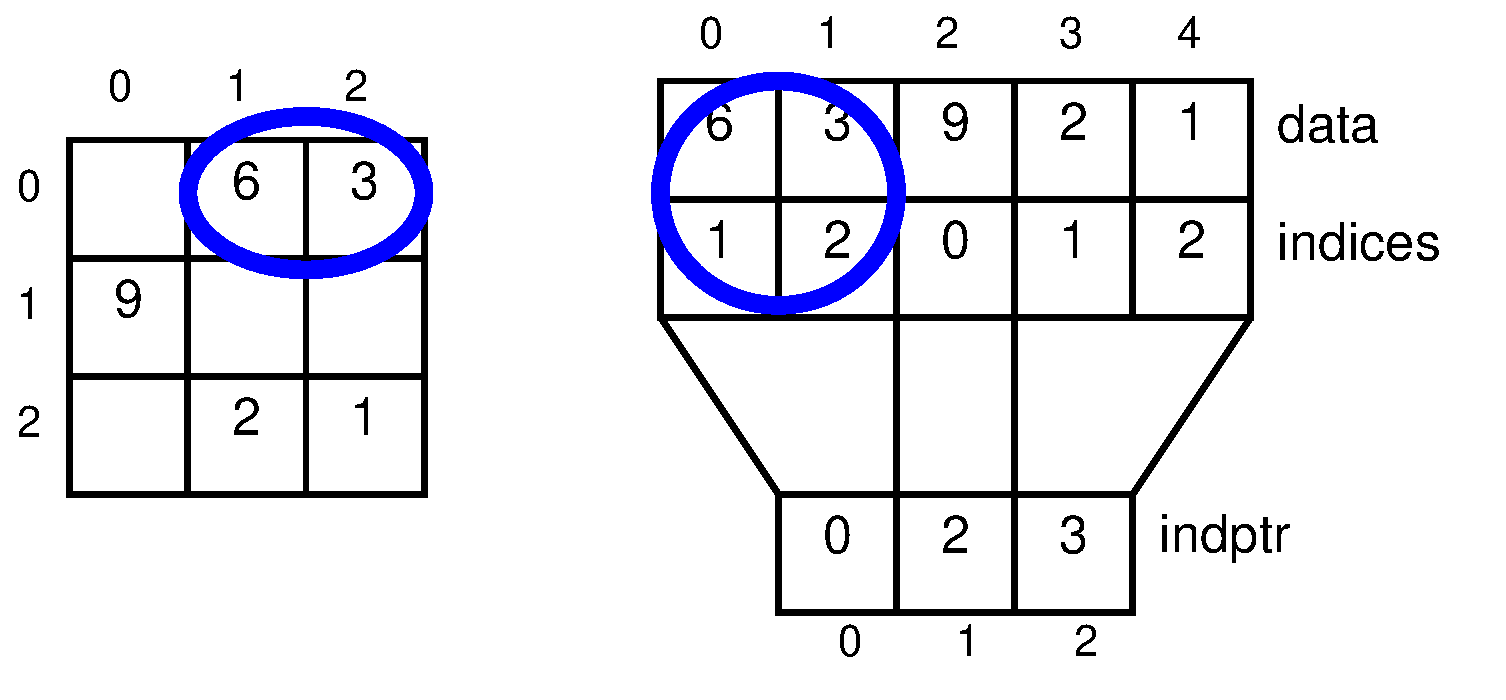
\includegraphics[scale=0.5]{stateofart/csr_format.eps}
\caption{Correspondence between a sparse matrix and its CSR counterpart.}
\label{fig:csr}
\end{figure}

\begin{itemize}
	\item a \emph{data} array containing all the non-zero values, where values from the same row appear sequentially, i.e. if the first row has 20 non-zero values, then the first 20 elements from this array belong to the first row;
	\item a \emph{indices} array contaning the column index of each non-zero value;
	\item a \emph{indptr} array containg a pointer to the first element in the \emph{data} and \emph{indices} arrays that belongs to each row, i.e. if the $i-th$ element (row) of \emph{indptr} is $k$ and it has 10 values, then all the elements from $k$ to $k + 5$ in \emph{data} belong to the $i-th$ row.
\end{itemize}

Within the algorithm's context, the three arrays are \emph{first\_edge} (previously \emph{indptr}, \emph{destination} (\emph{indices}) and \emph{weight} (\emph{data}). These three arrays can completely describe a graph. However, the algorithm uses an extra array \emph{outdegree} that can be deduced from the \emph{first\_edge} array. The length and purpose of each of this arrays is:
\begin{itemize}
	\item \emph{first\_edge} is an array of size $\|V\|$, where the \emph{i-th} element points to the first edge corresponding to the \emph{i-th} edge.
	\item \emph{outdegree} is an array of size $\|V\|$, where the \emph{i-th} element contains the number of edges attached to the \emph{i-th} edge.
	\item \emph{destination} is an array of size $\|E\|$, where the \emph{j-th} element points to the destination vertex of the \emph{j-th} edge.
	\item \emph{weight} is an array of size $\|E\|$, where the \emph{j-th} element contains the weight of the \emph{j-th} edge.
\end{itemize}

$V$ is the number of vertices and $E$ is the number of edges. The number of edges is duplicated to cover both directions. The edges in the \emph{destination} array are grouped together by the vertex they originate from, e.g. if edge $j$ is the first edge of vertex $i$ and this vertex has 3 edges, then edges $\{j,j+1,j+2\}$ are the outgoing edges of vertex $i$.



The algorithm consists on the following steps:

\begin{enumerate}
	\item 
\end{enumerate}


It should be noted, however, that this algorithm doe not support unconnected graphs, i.e., it is not able to output a forest of MSTs.
Upon contact, the author reported that a solution to that problem is, on the step of building the flag array, only mark a vertex if it is both the representative of its supervertex and has at least one neighbour.



\subsubsection{Exclusive scan} The \emph{scan} operation is one of the fundamental building block of parallel computing. 
Furthermore, two of the steps of the Borůvka variant of \cite{Sousa2015} are performed with an exclusive scan where the operation is a sum. 
To illustrate the functioning of the exclusive scan, let's consider the particular case where the operation of the scan is the sum and the identity (the value for which the operation produces the same output as the input) is naturally $0$. Let's further consider the input array to be the sequence $[0,1,2,3,4,5,6,7]$. Then the output will be $[0,0,1,3,5,8,13,19]$. The first element of the output will be the identity (if it were an inclusive scan, it would be the first element itself). The second element is the sum between the first element of the input array and the first element of the output array, the third element is the sum between the second element of the input array with second element of the output array, and so on.
This algorithm seems highly sequential in nature each element of the output array depends on the previous one. 
Still, two approaches exist to parallelize it:

% add refs and explain briefly
\begin{itemize} 
	\item Hillis and Steele
	\item Bleloch
\end{itemize}

%TODO fix refs
The two approaches focus on distinct efforts: the former focus on optimizing the number of steps while the later focus on optimizing the amount of work done.



%TODO the emphasis here must be GPGPU clustering and not MapReduce
%I have to find more literature regarding this
